\subsection{UC5 - Modifica vista magazzino}
\begin{figure}[H]
  \centering
  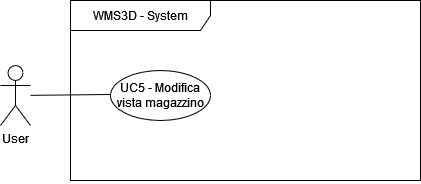
\includegraphics[width=0.8\textwidth]{UC_diagrams_1-10/UC5_sys.drawio.png}
   \caption{Diagramma UML UC5 - Modifica vista magazzino}
\end{figure}
\begin{figure}[H]
  \centering
  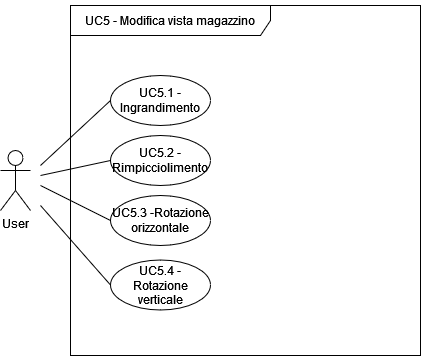
\includegraphics[width=0.8\textwidth]{UC_diagrams_1-10/UC5.drawio.png}
   \caption{Diagramma UML in dettaglio UC5 - Modifica vista magazzino}
\end{figure}
\begin{itemize}
    \item \textbf{Attori:} User.
    \item \textbf{Pre-condizione:}  L'utente sta visualizzando il magazzino in 3D [UC3].
    \item \textbf{Post-condizione:} L'utente visualizza il magazzino dal render 3D in maniera diversa.
    \item \textbf{Scenario Principale:}  L'utente può modificare la vista del render 3D del magazzino. In particolare, può visualizzare il magazzino più da vicino [UC5.1] o più da lontano [UC5.2], oppure può vedere il magazzino da una diversa angolazione, sia traslata orizzontalmente [UC5.3] sia verticalmente [UC5.4].
    \item \textbf{Generalizzazioni:} -
    \item \textbf{Estensioni:} -
\end{itemize}


\subsubsection{UC5.1 - Ingrandimento}
\begin{itemize}
    \item \textbf{Attori:} User.
    \item \textbf{Pre-condizione:}  L'utente sta visualizzando il magazzino in 3D [UC3].
    \item \textbf{Post-condizione:} L'utente osserva il magazzino nel render 3D più da vicino.
    \item \textbf{Scenario Principale:}  L'utente può visualizzare il magazzino più da vicino rispetto alla visualizzazione precedente.
    \item \textbf{Generalizzazioni:} -
    \item \textbf{Estensioni:} -
\end{itemize}


\subsubsection{UC5.2 - Rimpicciolimento}
\begin{itemize}
    \item \textbf{Attori:} User.
    \item \textbf{Pre-condizione:}  L'utente sta visualizzando il magazzino in 3D [UC3].
    \item \textbf{Post-condizione:} L'utente osserva il magazzino nel render 3D più da lontano.
    \item \textbf{Scenario Principale:}  L'utente può visualizzare il magazzino più da lontano [UC5.2] rispetto alla visualizzazione precedente.
    \item \textbf{Generalizzazioni:} -
    \item \textbf{Estensioni:} -
\end{itemize}


\subsubsection{UC5.3 - Rotazione orizzontale}
\begin{itemize}
    \item \textbf{Attori:} User.
    \item \textbf{Pre-condizione:}  L'utente sta visualizzando il magazzino in 3D [UC3].
    \item \textbf{Post-condizione:} L'utente osserva il magazzino nel render 3D da un'angolazione diversa, traslata orizzontalmente.
    \item \textbf{Scenario Principale:}  L'utente può visualizzare il magazzino da una diversa angolazione, spostata orizzontalmente rispetto alla visualizzazione precedente.
    \item \textbf{Generalizzazioni:} -
    \item \textbf{Estensioni:} -
\end{itemize}


\subsubsection{UC5.4 - Rotazione verticale}
\begin{itemize}
    \item \textbf{Attori:} User.
    \item \textbf{Pre-condizione:}  L'utente sta visualizzando il magazzino in 3D [UC3].
    \item \textbf{Post-condizione:} L'utente osserva il magazzino nel render 3D da un'angolazione diversa, traslata verticalmente.
    \item \textbf{Scenario Principale:} L'utente può visualizzare il magazzino da una diversa angolazione, spostata verticalmente rispetto alla visualizzazione precedente.
    \item \textbf{Generalizzazioni:} -
    \item \textbf{Estensioni:} -
\end{itemize}